\newpage
\section{Questão 12-17}

\begin{figure}[H]
	\centering
	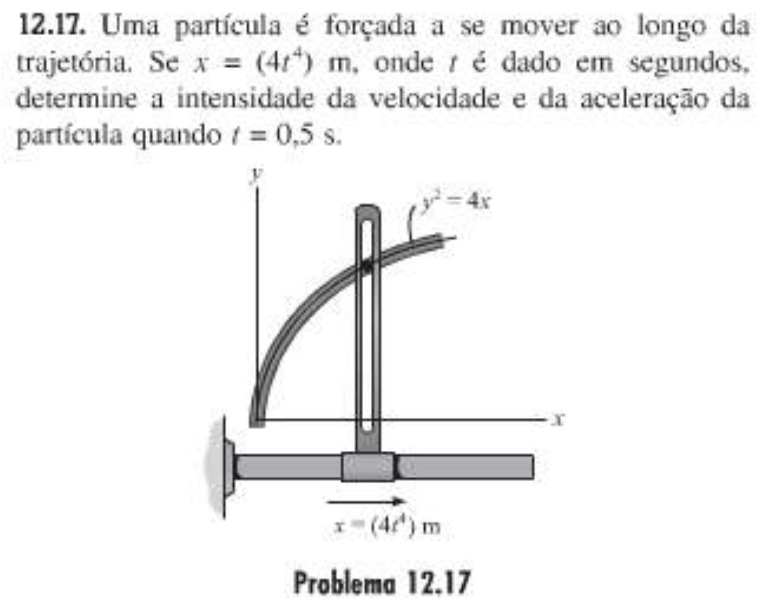
\includegraphics[width=.7\linewidth]{fundamentais/12-17.png}
\end{figure}

Nesta questão, analisamos o movimento de uma partícula cuja trajetória é definida por uma parábola \(y^2 = 4x\), com a posição em \(x\) dada como função do tempo \(t\). Determinamos as velocidades, acelerações e suas intensidades, bem como os valores numéricos no instante \(t = 0.5 \, \text{s}\).

\subsection*{Equação da Trajetória}
A equação da trajetória da partícula é definida como:
\[
y^2 = 4x,
\]
onde a posição \(x\) é dada por:
\[
x(t) = 4t^4.
\]

\subsection*{Cálculo das Derivadas para \(x\)}
A velocidade na direção \(x\) é obtida pela derivada de \(x(t)\) em relação ao tempo \(t\):
\[
v_x = \frac{dx}{dt} = \frac{d}{dt}\left(4t^4\right) = 16t^3.
\]

A aceleração na direção \(x\) é a derivada de \(v_x\):
\[
a_x = \frac{dv_x}{dt} = \frac{d}{dt}\left(16t^3\right) = 48t^2.
\]

\subsection*{Substituição de \(x\) na Equação da Trajetória}
Substituímos \(x(t)\) na equação da trajetória para encontrar \(y(t)\):
\[
y^2 = 4x \implies y^2 = 4(4t^4) \implies y = 4t^2.
\]

\subsection*{Cálculo das Derivadas para \(y\)}
A velocidade na direção \(y\) é:
\[
v_y = \frac{dy}{dt} = \frac{d}{dt}\left(4t^2\right) = 8t.
\]

A aceleração na direção \(y\) é:
\[
a_y = \frac{dv_y}{dt} = \frac{d}{dt}\left(8t\right) = 8.
\]

\subsection*{Intensidade da Velocidade}
A intensidade da velocidade é dada por:
\[
|\vec{v}| = \sqrt{v_x^2 + v_y^2}.
\]

Substituindo \(v_x\) e \(v_y\):
\[
|\vec{v}| = \sqrt{(16t^3)^2 + (8t)^2} = \sqrt{256t^6 + 64t^2}.
\]

\subsection*{Intensidade da Aceleração}
A intensidade da aceleração é dada por:
\[
|\vec{a}| = \sqrt{a_x^2 + a_y^2}.
\]

Substituindo \(a_x\) e \(a_y\):
\[
|\vec{a}| = \sqrt{(48t^2)^2 + (8)^2} = \sqrt{2304t^4 + 64}.
\]

\subsection*{Cálculos no Instante \(t = 0.5 \, \text{s}\)}
Substituímos \(t = 0.5 \, \text{s}\) nas equações para obter os valores numéricos:
\begin{itemize}
    \item Velocidade em \(x\): 
    \[
    v_x = 16t^3 \implies v_x = 16(0.5)^3 = 2.0 \, \text{m/s}.
    \]
    \item Velocidade em \(y\): 
    \[
    v_y = 8t \implies v_y = 8(0.5) = 4.0 \, \text{m/s}.
    \]
    \item Intensidade da velocidade:
    \[
    |\vec{v}| = \sqrt{256(0.5)^6 + 64(0.5)^2} \implies |\vec{v}| \approx 4.47 \, \text{m/s}.
    \]
    \item Intensidade da aceleração:
    \[
    |\vec{a}| = \sqrt{2304(0.5)^4 + 64} \implies |\vec{a}| \approx 14.42 \, \text{m/s}^2.
    \]
\end{itemize}

\subsection*{Resultados Finais}
\begin{itemize}
    \item Equações paramétricas:
    \[
    x(t) = 4t^4, \quad y(t) = 4t^2.
    \]
    \item Velocidade:
    \[
    v_x = 16t^3, \quad v_y = 8t.
    \]
    \item Aceleração:
    \[
    a_x = 48t^2, \quad a_y = 8.
    \]
    \item Intensidades:
    \[
    |\vec{v}| = \sqrt{256t^6 + 64t^2}, \quad |\vec{a}| = \sqrt{2304t^4 + 64}.
    \]
    \item Valores no instante \(t = 0.5 \, \text{s}\):
    \begin{itemize}
        \item \(v_x = 2.0 \, \text{m/s}\),
        \item \(v_y = 4.0 \, \text{m/s}\),
        \item \(|\vec{v}| \approx 4.47 \, \text{m/s}\),
        \item \(|\vec{a}| \approx 14.42 \, \text{m/s}^2\).
    \end{itemize}
\end{itemize}
